\documentclass[10pt,landscape,a4paper]{article}
\usepackage[utf8]{inputenc}
\usepackage[brazilian]{babel}
\usepackage[T1]{fontenc}
%\usepackage[LY1,T1]{fontenc}
%\usepackage{frutigernext}
%\usepackage[lf,minionint]{MinionPro}
\usepackage{tikz}
\usetikzlibrary{shapes,positioning,arrows,fit,calc,graphs,graphs.standard}
\usepackage[nosf]{kpfonts}
\usepackage[t1]{sourcesanspro}
\usepackage{graphics}
\usepackage{multicol}
\usepackage{wrapfig}
\usepackage[top=3mm,bottom=3mm,left=3mm,right=3mm]{geometry}
\usepackage[framemethod=tikz]{mdframed}
\usepackage{microtype}
\usepackage{pdfpages}

%\usepackage[shortlabels]{enumitem}

\let\bar\overline

\definecolor{myblue}{cmyk}{1,.72,0,.38}

\def\firstcircle{(0,0) circle (1.5cm)}
\def\secondcircle{(0:2cm) circle (1.5cm)}

\colorlet{circle edge}{myblue}
\colorlet{circle area}{myblue!5}

\tikzset{filled/.style={fill=circle area, draw=circle edge, thick},
    outline/.style={draw=circle edge, thick}}
    
\pgfdeclarelayer{background}
\pgfsetlayers{background,main}

\everymath\expandafter{\the\everymath \color{myblue}}
\everydisplay\expandafter{\the\everydisplay \color{myblue}}

\renewcommand{\baselinestretch}{.8}
\pagestyle{empty}

\global\mdfdefinestyle{header}{%
linecolor=gray,linewidth=1pt,%
leftmargin=0mm,rightmargin=0mm,skipbelow=0mm,skipabove=0mm,
}

\newcommand{\header}{
\begin{mdframed}[style=header]
\footnotesize
\sffamily
{\lage Cimat}\\
Eduardo~Borges~Lima.,~EQ/UFRJ~pg.\thepage~2019
\end{mdframed}
}

\makeatletter % Author: https://tex.stackexchange.com/questions/218587/how-to-set-one-header-for-each-page-using-multicols
\renewcommand{\section}{\@startsection{section}{1}{0mm}%
                                {.2ex}%
                                {.2ex}%x
                                {\color{myblue}\sffamily\small\bfseries}}
\renewcommand{\subsection}{\@startsection{subsection}{1}{0mm}%
                                {.2ex}%
                                {.2ex}%x
                                {\sffamily\bfseries}}



\def\multi@column@out{%
   \ifnum\outputpenalty <-\@M
   \speci@ls \else
   \ifvoid\colbreak@box\else
     \mult@info\@ne{Re-adding forced
               break(s) for splitting}%
     \setbox\@cclv\vbox{%
        \unvbox\colbreak@box
        \penalty-\@Mv\unvbox\@cclv}%
   \fi
   \splittopskip\topskip
   \splitmaxdepth\maxdepth
   \dimen@\@colroom
   \divide\skip\footins\col@number
   \ifvoid\footins \else
      \leave@mult@footins
   \fi
   \let\ifshr@kingsaved\ifshr@king
   \ifvbox \@kludgeins
     \advance \dimen@ -\ht\@kludgeins
     \ifdim \wd\@kludgeins>\z@
        \shr@nkingtrue
     \fi
   \fi
   \process@cols\mult@gfirstbox{%
%%%%% START CHANGE
\ifnum\count@=\numexpr\mult@rightbox+2\relax
          \setbox\count@\vsplit\@cclv to \dimexpr \dimen@-1cm\relax
\setbox\count@\vbox to \dimen@{\vbox to 1cm{\header}\unvbox\count@\vss}%
\else
      \setbox\count@\vsplit\@cclv to \dimen@
\fi
%%%%% END CHANGE
            \set@keptmarks
            \setbox\count@
                 \vbox to\dimen@
                  {\unvbox\count@
                   \remove@discardable@items
                   \ifshr@nking\vfill\fi}%
           }%
   \setbox\mult@rightbox
       \vsplit\@cclv to\dimen@
   \set@keptmarks
   \setbox\mult@rightbox\vbox to\dimen@
          {\unvbox\mult@rightbox
           \remove@discardable@items
           \ifshr@nking\vfill\fi}%
   \let\ifshr@king\ifshr@kingsaved
   \ifvoid\@cclv \else
       \unvbox\@cclv
       \ifnum\outputpenalty=\@M
       \else
          \penalty\outputpenalty
       \fi
       \ifvoid\footins\else
         \PackageWarning{multicol}%
          {I moved some lines to
           the next page.\MessageBreak
           Footnotes on page
           \thepage\space might be wrong}%
       \fi
       \ifnum \c@tracingmulticols>\thr@@
                    \hrule\allowbreak \fi
   \fi
   \ifx\@empty\kept@firstmark
      \let\firstmark\kept@topmark
      \let\botmark\kept@topmark
   \else
      \let\firstmark\kept@firstmark
      \let\botmark\kept@botmark
   \fi
   \let\topmark\kept@topmark
   \mult@info\tw@
        {Use kept top mark:\MessageBreak
          \meaning\kept@topmark
         \MessageBreak
         Use kept first mark:\MessageBreak
          \meaning\kept@firstmark
        \MessageBreak
         Use kept bot mark:\MessageBreak
          \meaning\kept@botmark
        \MessageBreak
         Produce first mark:\MessageBreak
          \meaning\firstmark
        \MessageBreak
        Produce bot mark:\MessageBreak
          \meaning\botmark
         \@gobbletwo}%
   \setbox\@cclv\vbox{\unvbox\partial@page
                      \page@sofar}%
   \@makecol\@outputpage
     \global\let\kept@topmark\botmark
     \global\let\kept@firstmark\@empty
     \global\let\kept@botmark\@empty
     \mult@info\tw@
        {(Re)Init top mark:\MessageBreak
         \meaning\kept@topmark
         \@gobbletwo}%
   \global\@colroom\@colht
   \global \@mparbottom \z@
   \process@deferreds
   \@whilesw\if@fcolmade\fi{\@outputpage
      \global\@colroom\@colht
      \process@deferreds}%
   \mult@info\@ne
     {Colroom:\MessageBreak
      \the\@colht\space
              after float space removed
              = \the\@colroom \@gobble}%
    \set@mult@vsize \global
  \fi}

\makeatother
\setlength{\parindent}{0pt}

\begin{document}
%	\raggedright
\footnotesize
%\small
\newlength{\mylen}
\setlength{\mylen}{0.5ex}
	\begin{multicols*}{5}		
		\section{Evolução dos materiais}
\subsection*{Idade da Pedra}
Materiais mais comuns: Polímeros (madeiram peles e fibras);Cerâmicos (Pedra)
\subsection*{Idade da Argila}
Materiais mais comuns: 
\subsection*{Idade do Cobre}
Materiais mais comuns: 
\subsection*{Idade do Bronze}
Materiais mais comuns: 
\subsection*{Idade do Ferro}
Materiais mais comuns: 
\section{Sociedade e Materiais}
Aumento significativo de tipos de materiais com o desenvolvimento industrial $\rhd$ Melhoria nos métodos de extração e produção \& Alterações nos materiais para formação de novos materiais (materiais avançados, compósitos)
\section{Classificação dos Materiais}
\subsection*{Metais}
Combinação de elementos metálicos, sendo possível a presença de não-metálicos (ex: aço-carbono).Algumas propriedades relacionadas à presença de elétrons livres (ex: bons condutores de calor e eletricidade).Resistentes e deformáveis: extenso uso em aplicações estruturais.
Suscetível a corrosão.

Possui boa condutividade térmica e elétrica.
\subsection*{Cerâmicos}
ligações de metais e não-metais. Isolantes térmicos e elétricos. Podem ser resistentes a altas temperaturas e a ambientes agressivos. Ex: óxidos, nitretos, carbetos.
Resistentes a corrosão.

Possui boa condutividade térmica e variada condutividade elétrica.
\subsection*{Polímeros}
polímeros:compostos orgânicos. Baixa densidade; altamente deformáveis. (C, H e não-metálicos)
Degrada com solventes, altas temperaturas.

Possui baixa condutividade térmica e elétrica.
\subsection*{Compósitos}
Compósitos: dois ou mais tipos de materiais unidos de forma a produzir um material com características específicas. Projetados para apresentar uma combinação das melhores características de cada um dos componentes.

\subsection*{Materiais avançados}
Usoemaplicaçõesde ponta(altatecnologia). Nãonecessariamentesãonovosmateriais. Podemser tradicionais, com otimizaçãodas propriedades.

\begin{itemize}
		
	\setlength{\parskip}{0pt}
	\setlength{\itemsep}{0pt plus 1pt}
	
\item Alto desempenho
\item Baixo peso e alta resistência
\item Resistência a diversas condições de serviço
\item Ambientalmente corretos
\item Facilmente recicláveis
\end{itemize}
Ex: polímero reforçado com fibra de vidro usado como armadura para estruturas em concreto armado


\section{Classificação dos Materiais}

\subsection*{Qaunto a Estrutura}

\begin{itemize}
		
	\setlength{\parskip}{0pt}
	\setlength{\itemsep}{0pt plus 1pt}
	
	\item Ligações atômicas
	
	\begin{itemize}
			
		\setlength{\parskip}{0pt}
		\setlength{\itemsep}{0pt plus 1pt}
		
		\item Metálica
		\item covalente
		\item iônica
	\end{itemize}

	\item Tipo de Estrutura
	\begin{itemize}
			
		\setlength{\parskip}{0pt}
		\setlength{\itemsep}{0pt plus 1pt}
		
		\item Amorfa
		\item Cristalina
		\item Molecular
	\end{itemize}
\end{itemize}


\subsection*{Propriedades Mecânicas}
\begin{itemize}
		
	\setlength{\parskip}{0pt}
	\setlength{\itemsep}{0pt plus 1pt}
	
	\item dutilidade
	\item elasticidades
	\item dureza
	\item tenacidade
\end{itemize}

\subsection*{Propriedades Químicas e Físicas}
\begin{itemize}
		
	\setlength{\parskip}{0pt}
	\setlength{\itemsep}{0pt plus 1pt}
	
\item	ponto de fusão
\item	calor específico
\item	condutividade (térmica e elétrica)
\item 	Propriedades magnéticas
\item 	Propriedades ópticas
\item 	Iteração com o ambiente: oxidação 
\end{itemize}

\subsection*{Modificação das Propriedades}
\begin{itemize}
		
	\setlength{\parskip}{0pt}
	\setlength{\itemsep}{0pt plus 1pt}
	
	\item Tratamentos térmicos
	\item tratamento de superfície
	\item Tratamentos mecânicos
\end{itemize}


\section{COMPOSIÇÃO QUÍMICA x PROPRIEDADES FÍSICAS}
Exemplo 1: alteração de cor de um mesmo mineral

CORÍNDON:mineral à base de óxido de alumínio (Al2O3)
Chama-se safira qualquer variedade de corindon, de qualidade gemológica, que não seja vermelha (rubi)

Exemplo 2: Alteração da compatibilidade química com o meio ambiente.
Aço patinável (CORTEN): aço com adição de cobre que forma uma pátina, reduzindo o processo corrosivo. Muito usado na construção civil.



\section{ESTRUTURA CRISTALINA x PROPRIEDADES FÍSICAS}
CaCO3

Mármore (calcita -romboédrico)

Conchas (aragonita -ortorrômbico)

\section{TIPO DE LIGAÇÃO QUÍMICA x PROPRIEDADES FÍSICAS}

O tipo de ligação iônica está intimamente ligada com as características físico-química dos materiais.

Temos que:
\subsection*{Ligações Metálicas}
Favorecem a condutividade térmica e elétrica

\subsection*{Ligações Covalentes}
Aparecem em matérias com características isolantes. 


\section{Materiais de Construção}

\subsection*{Escolha do Material}

Etapas básicas

\begin{itemize}
	
\setlength{\parskip}{0pt}
\setlength{\itemsep}{0pt plus 1pt}

\item relacionar experiências prévias para o serviço em questão
\item relacionar e colocar em ordem de prioridade todos os parâmetros que podem influenciar na escolha
\item estabelecer as características que se deseja para o material ideal ao serviço
\item realizar testes, comparando os materiais que possam ser usados otimizando o custo total.

\end{itemize}

Definição da categoria do material: metal, cerâmico, polímero ou compósito

\subsection*{Como selecionar um material?}

Condições operacionais
\begin{itemize}
	
	\setlength{\parskip}{0pt}
	\setlength{\itemsep}{0pt plus 1pt}
	
\item Custo/benefício (indústria de massa ou de grande exigência tecnológica?)
\item Propriedades requeridas
\item Degradação no meio
\item Solicitação mecânica
\item Resistência/peso
\end{itemize}

\subsection*{Quais fatores influenciam na escolha dos materiais para determinado serviço ou aplicação industrial?}

\begin{itemize}
	\item Propriedades físicas e químicas 
	\item Características operacionais
	\item Fabricação, disponibilidade e custo
	
\end{itemize}


\section{Propriedades físicas e químicas}

\subsection*{Propriedades mecânicas}
Limites de escoamento e de resistência, dutilidade, resistência à fadiga e fluência, temperatura de transição dútil-frágil, módulo de elasticidade.

\subsection{Outras propriedades físicas}
densidade, calor específico,expansão térmica,condutividade,propriedades magnéticas e elétricas.


\subsection*{Propriedades químicas}
oxidação, flamabilidade,toxicidade.

\section{Características operacionais}

\subsection*{temperatura}
\subsection*{natureza dos fluidos em contato com material}
(composição química, concentração, pH, caráter oxidante ou redutor, presença de contaminantes, pressão, velocidade do fluido, flamabilidade, toxidez). Necessário avaliar alterações em cada um destes fatores ao longo do tempo de serviço.

\subsection*{presença de resíduos oriundos de processos corrosivos}
ex: alguns materiais como o chumbo são resistentes à corrosão porém geram resíduos tóxidos, limitando seu uso.

\section{Fabricação,disponibilidade e custo}


\subsection*{Fatores críticos na seleção:} facilidade de fabricação e forma de apresentação. Ex:espessura de chapas e formato(tubos ou tarugos)
Custo/benefício: custo direto do material, tempo de vida útil e custos indiretos (paradas para reparos ou reposição dos equipamentos).
Tempo de vida útil compatível com tempo previsto de operação.
Relação direta com segurança (acidentes e falhas)
Furos em tubulações.
Aço inox 304 no lugar de aço-C.
Aço-carbono disponível em inúmeras formas de fabricação.

\vspace{150px}

\section{Estrutura Cristalina}

\subsection*{Material Amorfo X Cristalino}
O material CRISTALINO possui arranjo mais uniforme e as moléculas está direcionadas de forma a apresentarem um densidade molecular maior. 

O material AMORFO possui suas moléculas dispostas de forma mais aleatória e a densidade molecular dessa região é menor.


\subsection*{CRISTALINIDADE} Arranjo interno ordenado das partículas segundo um modelo tridimensional, característico do estado sólido. Em muitos corpos a cristalinidade é evidenciada por faces e simetria externa, indicando um arranjo ordenado dos átomos. Exames em raios X(1912) estudo de substâncias inorgânicas.

\subsection*{CRISTALOGRAFIA} Estudo dos corpos sólidos que possuem estrutura cristalina e das leis que governam seu crescimento, forma externa e interna. É instrumento fundamental na química, física, metalurgia e no estudos das cerâmicas, refratários, semicondutores, gemas sintéticas, etc.


\subsection*{CÉLULAS UNITÁRIAS} para a maioria dos cristais, as células unitárias podem ser representadas por geometrias específicas. Mais do que uma célula unitária pode ser escolhida para representar o cristal. Geralmente, escolhe-se a que apresenta o maior grau de simetria geométrica.



\subsection*{SISTEMAS CRISTALINOS} Qualquer empacotamento atômico deverá se encaixar em um dos sete principais tipos de cristais, que estão intimamente associados com o modo pelo qual o espaço pode ser dividido em volumes iguais, pela interseção de superfícies planas.
Existem diferentes estruturas cristalinas possíveis. É conveniente dividi-las em grupos de acordo com as configurações das células unitárias e/ou os arranjos atômicos. Para criar todos os tipos de redes são necessários sete tipos distintos de células cristalinas.


\section{Células unitárias e Sistemas cristalinos}

Parâmetros de rede cristalina:
\begin{itemize}
	\item a,b,c - comprimentos dos lados do paralelepípedo
	\item $ \alpha$, $\beta$, $\gamma $ - ângulos entre os eixos
\end{itemize}

$\gamma $





Com base nestes parâmetros de rede, tem-se que existem 7 diferentes combinações possíveis entre a,b,c e $\alpha, \beta, \gamma $ cada um representando um sistema cristalino.


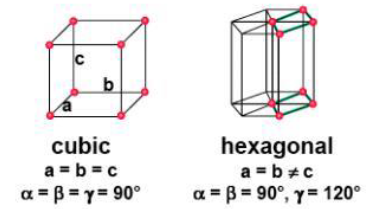
\includegraphics[scale=0.5,trim={0 0 0 0}]{figures/crist1}
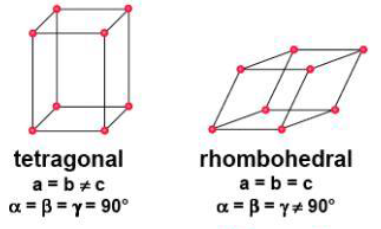
\includegraphics[scale=0.5,trim={0 0 0 0}]{figures/crist2}
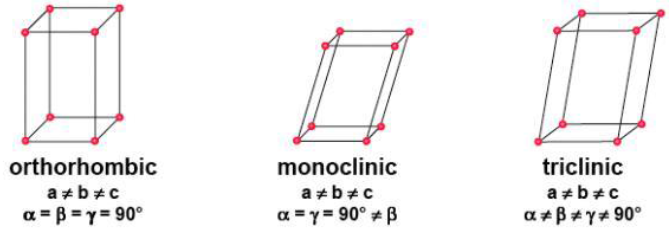
\includegraphics[scale=0.3,trim={0 0 0 0}]{figures/crist3}


O maior grau de simetria aparece no sistema cúbico e o menor grau é visto no sistema triclínico.

\subsection*{Variações na célula unitária básica}

As possíveis redes podem ser descritas por 14 células unitárias (A.J. Bravais).
Em algumas células unitárias existem alguns tipos básicos: simples, de corpo centrado e de faces centradas.
 
 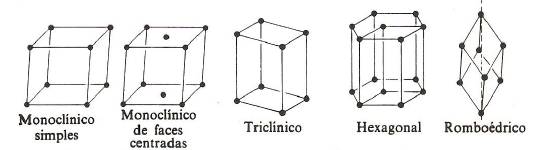
\includegraphics[scale=0.5,trim={0 0 0 0}]{figures/var1}
 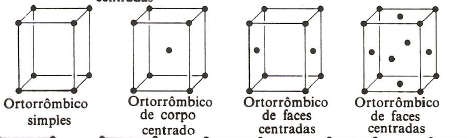
\includegraphics[scale=0.45,trim={0 0 0 0}]{figures/var2}
 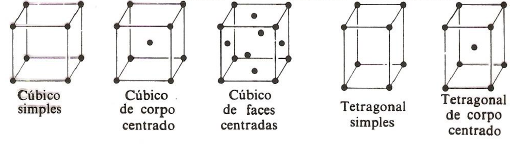
\includegraphics[scale=0.5,trim={0 0 0 0}]{figures/var3}

"C:/Windows/System32/cmd.exe" "C:/Users/OdnSpceMaker/Documents/GitHub/commit2.bat"


 BAHHHH

Fatores Criticos na bunda

quere qeu erq

qeerer
 
%\subsection*{Aussage}
%Eine Aussage ist ein Satz, der entweder wahr oder falsch ist, also nie beides zugleich.
%Wahre Aussagen haben den Wahrheitswert $w$ und falsche Aussagen den
%Wahrheitswert $f$.
%\subsection*{Belegung von Variablen}
%Sei $\mathcal{A}_B(F) = f$.
%Dann ist stets $\mathcal{A}_B(F\Rightarrow G) = w$
%\subsection*{Formelbeweis über Belegung}
%Wenn $F \wedge G$ eine Tautologie ist, dann (und nur dann) ist $F$ eine Tautologie und $G$ auch.
%Hinweis: In dem Lemma stecken zwei Teilaussagen, die beide zu beweisen sind:
%1. Wenn $F \wedge G$ eine Tautologie ist, dann ist $F$ eine Tautologie und $G$ auch.
%2. Umgekehrt: Sind $F$ und $G$ Tautologien, dann ist auch $F \wedge G$ eine.
%\emph{Beweis.}
%1. Annahme: $F \wedge G$ sei eine Tautologie.
%Dann: Für jede Belegung $B$ wertet $F \wedge G$ zu wahr aus.
%Dann: Das ist nur der Fall, wenn sowohl $F$ als auch $G$ (für jedes $B$) zu wahr auswerten.
%Dann: Für jede Belegung $B$ wertet $F$ zu wahr aus. Und:
%Für jede Belegung $B$ wertet $G$ zu wahr aus.
%Dann: $F$ ist Tautologie und $G$ ist Tautologie.
%2. Annahme: $F$ ist Tautologie und $G$ ist Tautologie.
%Dann: Für jede Belegung $B_1$ wertet $F$ zu wahr aus. Und: Für jede Belegung $B_2$ wertet $G$ zu wahr aus.
%Dann: Für jede Belegung $B$ wertet $F \wedge G$ zu wahr aus.
%Dann: $F \wedge G$ ist eine Tautologie.
%\subsection*{Äquivalenz und Folgerung}
%$p\equiv q$ gilt genau dann, wenn sowohl $p\models q$ als auch $q\models p$ gelten. \emph{Beweis.}
%$p\equiv q$ GDW $p\Leftrightarrow q$ ist Tautologie nach Def. von $\equiv$
%GDW $(p\Rightarrow q) \wedge (q\Rightarrow p)$ ist Tautologie
%GDW $(p\Rightarrow q)$ ist Tautologie und $(q\Rightarrow p)$ ist Tautologie
%GDW $(p\models q)$ gilt und $q\models p$ gilt.
%\subsection*{Substitution}
%Ersetzt man in einer Formel eine beliebige Teilformel $F$ durch eine logisch äquivalente
%Teilformel $F'$, so verändert sich der Wahrheitswerteverlauf der Gesamtformel nicht.
%Man kann Formeln also vereinfachen, indem man Teilformeln durch äquivalente
%(einfachere) Teilformeln ersetzt.
%\subsection*{Universum}
%Die freien Variablen in einer Aussagenform können durch Objekte aus einer als
%Universum bezeichneten Gesamtheit wie $\mathbb{N},\mathbb{R},\mathbb{Z},\mathbb{Q}$ ersetzt werden.
%\subsection*{Tautologien}
%$(p\wedge q)\Rightarrow p$\text{ bzw. }$p\Rightarrow (p\vee q)$\\
%$(q\Rightarrow p)\vee (\neg q\Rightarrow p)$\\
%$(p\Rightarrow q)\Leftrightarrow (\neg p\vee q)$\\
%$(p\Rightarrow q)\Leftrightarrow (\neg q\Rightarrow\neg p)$ \hfill\text{(Kontraposition)}\\
%$(p\wedge (p\Rightarrow q))\Rightarrow q$ \hfill\text{(Modus Ponens)}\\
%$((p\Rightarrow q)\wedge (q\Rightarrow r))\Rightarrow (p\Rightarrow r)$\\
%$((p\Rightarrow q)\wedge (p\Rightarrow r))\Rightarrow (p\Rightarrow (q\wedge r))$\\
%$((p\Rightarrow q)\wedge (q\Rightarrow p))\Leftrightarrow (p\Leftrightarrow q)$
%\subsection*{Nützliche Äquivalenzen}
%Kommutativität:\\
%$(p \wedge q) \equiv (q \wedge p)$\\
%$(p \vee q) \equiv (q \vee p)$\\
%Assoziativität:\\
%$(p \wedge (q \wedge r)) \equiv ((p \wedge q) \wedge r)$\\
%$(p \vee (q \vee r)) \equiv ((p \vee q) \vee r)$\\
%Distributivität:\\
%$(p \wedge (q \vee r)) \equiv ((p \wedge q) \vee (p \wedge r))$\\
%$(p \vee (q \wedge r)) \equiv ((p \vee q) \wedge (p \vee r))$\\
%Idempotenz:\\
%$(p \wedge p) \equiv p$\\
%$(p \vee p) \equiv p$\\
%Doppelnegation:\\
%$\neg (\neg p) \equiv p$\\
%de Morgans Regeln:\\
%$\neg (p \wedge q) \equiv ((\neg p) \vee (\neg q))$\\
%$\neg (p \vee q) \equiv ((\neg p) \wedge (\neg q))$\\
%Definition Implikation:\\
%$(p \Rightarrow q) \equiv (\neg p \vee q)$\\
%Tautologieregeln:\\
%$(p \wedge q) \equiv p$\hfill (falls $q$ eine Tautologie ist)\\
%$(p \vee q) \equiv q$\\
%Kontradiktionsregeln:\\
%$(p \wedge q) \equiv q$\hfill (falls $q$ eine Kontradiktion ist)\\
%$(p \vee q) \equiv p$\\
%Absorptionsregeln:\\
%$(p \wedge (p \vee q)) \equiv p$\\
%$(p \vee (p \wedge q)) \equiv p$\\
%Prinzip vom ausgeschlossenen Dritten:\\
%$p \vee (\neg p) \equiv w$\\\
%Prinzip vom ausgeschlossenen Widerspruch:\\
%$p \wedge (\neg p) \equiv f$
%\subsection*{Äquivalenzen von quant. Aussagen}
%Negationsregeln:\\
%$\neg\forall x:p(x)\equiv\exists x:(\neg p(x))$\\
%$\neg\exists x:p(x)\equiv\forall x:(\neg p(x))$\\
%Ausklammerregeln:\\
%$(\forall x:p(x)\wedge\forall y:q(y))\equiv\forall z:(p(z)\wedge q(z))$\\
%$(\exists x:p(x)\wedge\exists y:q(y))\equiv\exists z:(p(z)\wedge q(z))$\\
%Vertauschungsregeln\\
%$\forall x\forall y:p(x,y)\equiv\forall y\forall x:p(x,y)$\\
%$\exists x\exists y:p(x,y)\equiv\forall y\exists x:p(x,y)$
%\subsection*{Äquivalenzumformung}
%Wir demonstrieren an der Formel $\neg (\neg p \wedge q) \wedge (p \vee q)$, wie man mit Hilfe der
%aufgelisteten logischen Äquivalenzen tatsächlich zu Vereinfachungen kommen kann:\\
%$\phantom{{}\equiv{}} \neg (\neg p \wedge q) \wedge (p \vee q)$\\
%$\equiv (\neg (\neg p) \vee (\neg q)) \wedge (p \vee q)$\hfill de Morgan\\
%$\equiv (p \vee (\neg q)) \wedge (p \vee q)$\hfill Doppelnegation\\
%$\equiv p \vee ((\neg q) \wedge q)$\hfill Distributivtät v.r.n.l.\\
%$\equiv p \vee (q \wedge (\neg q))$\hfill Kommutativtät\\
%$\equiv p \vee f$\hfill Prinzip v. ausgeschl. Widerspruch\\
%$\equiv p$\hfill Kontradiktionsregel
%\subsection*{Quantifizierte Aussagen}
%Sei $p(x)$ eine Aussageform über dem Universum $U$.
%$\exists x : p(x)$ ist wahr genau dann, wenn ein $u$ in $U$ existiert, so dass $p(u)$ wahr ist.
%$\forall x : p(x)$ ist wahr genau dann, wenn $p(u)$ für jedes $u$ aus $U$ wahr ist.

		%\section{Mengenlehre}
\subsection*{Teilmenge und Obermenge}
Eine Menge $B$ heißt Teilmenge einer Menge $A$ genau dann,
wenn jedes Element von $B$ auch ein Element von $A$ ist ($B\subseteq A\Leftrightarrow\forall x:x\in B\Rightarrow x\in A$).
$A$ heißt dann Obermenge von $B$. Eine Menge $B$ heißt echte Teilmenge von $A$ ($B\subset A$), falls gilt $B\subseteq A\wedge B\neq A$
\subsection*{Grundlegende Mengenoperationen}
Seien $M, N$ Mengen und sei $U$ die Grundmenge.\\
Vereinigungsmenge:\\
$M\cup N:=\{x\mid x\in M\vee x\in N\}$\\
Schnittmenge:\\
$M\cap N:=\{x\mid x\in M\wedge x\in N\}$\\
Differenz:\\
$M\setminus N:=\{x\mid x\in M\wedge x\notin N\}$\\
Disjunkte Menge: $M\cap N=\emptyset$
\subsection*{Potenzmenge}
Sei $M$ eine Menge. Die Menge aller Teilmengen von $M$ heißt Potenzmenge von $M$ und
wird $\mathcal{P}(M)$ notiert: $\mathcal{P}(M):=\{X\mid X\subseteq M\}$\\
\emph{Beispiel:}\\
$\mathcal{P}(\{a,b\})=\{\emptyset,\{a\},\{b\},\{a,b\}\}$\\
$\mathcal{P}(\emptyset)=\{\emptyset\}$\\
$\mathcal{P}(\{\emptyset\})=\{\emptyset,\{\emptyset\}\}$\\
$\mathcal{P}(\mathcal{P}(\mathcal{P}(\emptyset)))=\{\emptyset,\{\emptyset\},\{\{\emptyset\}\},\{\emptyset,\{\emptyset\}\}\}$
\subsection*{Hassediagramm}
\begin{wrapfigure}[9]{r}{.46\linewidth}
\vspace{-20pt}
\hspace{-0pt}
\begin{tikzpicture}[scale=0.4]
  \node (max) at (0,4) {$\{x,y,z\}$};
  \node (a) at (-2,2) {$\{x,y\}$};
  \node (b) at (0,2) {$\{x,z\}$};
  \node (c) at (2,2) {$\{y,z\}$};
  \node (d) at (-2,0) {$\{x\}$};
  \node (e) at (0,0) {$\{y\}$};
  \node (f) at (2,0) {$\{z\}$};
  \node (min) at (0,-2) {$\emptyset$};
  \draw (min) -- (d) -- (a) -- (max) -- (b) -- (f)
  (e) -- (min) -- (f) -- (c) -- (max)
  (d) -- (b);
  \draw[preaction={draw=white, -,line width=6pt}] (a) -- (e) -- (c);
\end{tikzpicture}
\end{wrapfigure}
Man kann die Inklusionsbeziehungen aller Teilmengen in Form eines Hasse-Diagramms veranschaulichen. Das Hasse-Diagramm für $\mathcal{P}(\{x,y,z\})$ lässt sich dann wie folgt darstellen:
\subsection*{Venn-Diagramm}
\begin{tikzpicture}[scale=.45]
    \begin{scope}
        \clip \firstcircle;
        \fill[filled] \secondcircle;
    \end{scope}
    \draw[outline] \firstcircle node {$A$};
    \draw[outline] \secondcircle node {$B$};
    \node[anchor=south] at (current bounding box.north) {$A \cap B$};
\end{tikzpicture}
%Set A or B but not (A and B) also known a A xor B
\begin{tikzpicture}[scale=.45]
\hspace{-.5cm}
    \draw[filled, even odd rule] \firstcircle node {$A$}
                                 \secondcircle node{$B$};
    \node[anchor=south] at (current bounding box.north) {$\overline{A \cap B}$};
\end{tikzpicture}
% Set A or B
\begin{tikzpicture}[scale=.45]
    \draw[filled] \firstcircle node {$A$}
                  \secondcircle node {$B$};
    \node[anchor=south] at (current bounding box.north) {$A \cup B$};
\end{tikzpicture}
% Set A but not B
\hspace{.5cm}
\begin{tikzpicture}[scale=.45]
    \begin{scope}
        \clip \firstcircle;
        \draw[filled, even odd rule] \firstcircle node {$A$}
                                     \secondcircle;
    \end{scope}
    \draw[outline] \firstcircle
                   \secondcircle node {$B$};
    \node[anchor=south] at (current bounding box.north) {$A\setminus B$};
\end{tikzpicture}
\subsection*{Operationen auf Mengenfamilien}
Sei $\mathcal{F}=\{\{1,2,3,4\},\{3,4,5,6\}\}$ Mengenfamilie.
Vereinigung aller Mengen aus $\mathcal{F}$:\\
$\bigcup\mathcal{F}=\{1,2,3,4,5,6\}$\\
Durchschnitt aller Mengen aus $\mathcal{F}$:\\
$\bigcap\mathcal{F}=\{3,4\}$
\subsection*{Kartesisches Produkt}
Seien $A,B$ Mengen, dann ist das kartesische Produkt (Kreuzprodukt)
von $A$ und $B$ definiert als: $A\times B:=\{(a,b)\mid a\in A\wedge b\in B\}$. 
$A\times B$ ist die Menge aller geordneten Paare von $A$ und $B$.\\
\emph{Hinweis:}\\
$(a,b)=(c,d)\Leftrightarrow a=c\wedge b=d$\\
$A\times\emptyset=\emptyset\times A=\emptyset$\\
$A\times B\neq B\times A$\\
\emph{Beispiel:}\\
$\{1,2\}\times\{3,4\}=\{(1,3),(1,4),(2,3),(2,4)\}$\\
$\{3,4\}\times\{1,2\}=\{(3,1),(3,2),(4,1),(4,2)\}$
\subsection*{Rechenregeln für Mengenoperationen}
Assoziativgesetze:\\
$(A\cup B)\cup C=A\cup (B\cup C)$\\
$(A\cap B)\cap C=A\cap (B\cap C)$\\
Kommutativgesetze:\\
$A\cup B=B\cup A$\\
$A\cap B=B\cap A$\\
Distributivgesetze:\\
$(A\cup B)\cap C=(A\cap C)\cup (B\cap C)$\\
$(A\cap B)\cup C=(A\cup C)\cap (B\cup C)$\\
de Morganschen Gesetze (Differenz):\\
$A\setminus (B\cup C)=(A\setminus B)\cap (A\setminus C)$\\
$A\setminus (B\cap C)=(A\setminus B)\cup (A\setminus C)$\\
de Morganschen Gesetze (Komplement):\\
$\bar{A\cup B}=\bar{A}\cap\bar{B}$\\
$\bar{A\cap B}=\bar{A}\cup\bar{B}$\\
Absorptionsgesetze:\\
$A\cap (A\cup B)=A$\\
$A\cup (A\cap B)=A$\\
Idempotenzgesetze:\\
$A\cap A=A$\\
$A\cup A=A$\\
Komplementgesetze ($G$ ist Grundmenge):\\
$A\cap\bar{A}=\emptyset$\\
$A\cup\bar{A}=G$
		%\section{Relationen}
\subsection*{Binäre Relation}
Eine binäre Relation $R$ ist eine Menge von Paaren $(a,b)\in A\times B$.\\
$aRb\Leftrightarrow (a,b)\in R$ bzw. $a(\neg R)b\Leftrightarrow (a,b)\notin R$\\
\emph{Beispiele:}\\
Teilerrelation ($nTm$): $P_3:=\{(n,m+3)\mid n,m\in\mathbb{N}\}=\{(1,4),(2,5),(3,6),...\}$\\
Relation $\subset$ über $\mathcal{P}(M)$ für $M=\{1,2\}$:\\
$\{(\emptyset ,\{1\}),(\emptyset ,\{2\}),(\emptyset ,\{1,2\}),(\{1\},\{1,2\}),\\(\{2\} ,\{1,2\})\}$
\subsection*{Inverse Relation}
Sei $R\subseteq A\times B$. Die inverse Relation zu $R$ ist $R^{-1}=\{(y,x)\in B\times A\mid (x,y)\in R\}$. Also ist $R^{-1}\subseteq B\times A$.\\
\emph{Beispiel:} Sei $R=\{(1,a),(1,c),(3,b)\}$ dann ist $R^{-1}=\{(a,1),(c,1),(b,3)\}$
\subsection*{Komposition}
Seien $R\subseteq M_1\times M_2$ und $S\subseteq M_2\times M_3$ zweistellige Relationen.
Die Verknüpfung $(R\circ S)\subseteq (M_1\times M_3)$ heißt Komposition der Relationen $R,S$.\\
$R\circ S:=\{(x,z)\mid\exists y\in M_2:(x,y)\in R\wedge (y,z)\in S\}$\\
\emph{Beispiel:} Sei $R=\{(1,2),(2,5),(5,1)\}$, dann ist $R^2=R\circ R=\{(1,5),(2,1),(5,2)\}$\\
Sei $R\subseteq\mathbb{N}\times\mathbb{N}$ mit $(n,m)\in R\Leftrightarrow m=3n$ und
$S\subseteq\mathbb{N}\times\mathbb{Z}$ mit $(n,z)\in S\Leftrightarrow z=-n$. Dann ist $R\circ S=\{(n,z)\mid z=-3n\}\subseteq\mathbb{N}\times\mathbb{Z}$
\subsection*{Eigenschaften von Operationen}
$(R\cup S)^{-1}=R^{-1}\cup S^{-1}$\\
$(R\cap S)^{-1}=R^{-1}\cap S^{-1}$\\
$(R\circ S)^{-1}=S^{-1}\circ R^{-1}$\\
$(R\cap S)\circ T\subseteq (R\circ T)\cap (S\circ T)$\\
$T\circ (R\cap S)\subseteq (T\circ R)\cap (T\circ S)$\\
$(R\cup S)\circ T = (R\circ T)\cup (S\circ T)$\\
$T\circ (R\cup S) = (T\circ R)\cup (T\circ S)$
\subsection*{Eigenschaften von Relationen}
Reflexiv: $\forall a\in A:(a,a)\in R$\\
Symmetrisch: $\forall a,b\in A:(a,b)\in R\Rightarrow (b,a)\in R$\\
Antisymm.: $\forall a,b\in A:(a,b)\in R\wedge (b,a)\in R\Rightarrow a=b$\\
Transitiv: $\forall a,b,c\in A:(a,b)\in R\wedge (b,c)\in R\Rightarrow (a,c)\in R$\\
Total: $\forall a,b \in A: (a,b)\in R\vee (b,a)\in R$\\
Irreflexiv: $\forall a\in A: (a,a)\notin R$\\
Asymm.: $\forall a,b\in A:(a,b)\in R\Rightarrow (b,a)\notin R$\\
Alternativ: $\forall a,b\in A:(a,b)\in R\oplus (b,a)\in R$\\
Rechtseind.: $\forall a\in A:(a,b)\in R\wedge (a,c)\in R\Rightarrow b=c$\\
Linkseind.: $\forall a\in A:(b,a)\in R\wedge (c,a)\in R\Rightarrow b=c$\\
Eindeutig: $R$ ist recht- und linkseindeutig.\\
Linkstotal: $\forall a\in A\exists b\in B:(a,b)\in R$\\
Rechtstotal: $\forall b\in B\exists a\in A:(a,b)\in R$
\subsection*{Äquivalenzrelation}
Ist eine Relation $\sim$ reflexiv, symmetrisch und transitiv, heißt sie Äquivalenzrelation.
\subsection*{Äquivalenzklassen}
Gegeben eine Äquivalenzrelation $R$ über der Menge $A$.
Dann ist für $a\in A$: $[a]_R=\{x\mid (a,x)\in R\}$ die Äquivalenzklasse von $a$.\\
(Äquivalente Elemente kommen in die gleiche Menge)\\
\emph{Beispiel (Restklassen):}\\
$[4]=\{n\mid n\mod 3=4 \mod 3\}=[1]$\\
$[5]=\{n\mid n\mod 3=5 \mod 3\}=[2]$\\
$[6]=\{n\mid n\mod 3=6 \mod 3\}=[3]$
\subsection*{Zerlegungen, Partition}
Eine Zerlegung (Partition) $\mathcal{Z}$ ist eine Einteilung von $A$ in nicht leere, paarweise
elementfremde Teilmengen, deren Vereinigung mit $A$ übereinstimmt.\\
\emph{Beispiel:} Sei $A=\{1,2,3,...,10\}$. Dann ist $\mathcal{Z_1}=\{\{1,3\},\{2,5,9\},\{4,10\},\{6,7,8\}\}$
\subsection*{Abschluss einer Relation}
$R_\phi^*$ bildet die fehlenden Relationen mit der Eigenschaft $\phi$, also alle Kombinationen aus $A$, die noch nicht in $R$ sind.\\
\emph{Beispiel:}\\
Sei $A=\{1,2,3\}$ und $R=\{(1,2),(2,3),(3,3)\}$. 
Dann ist $R_{refl}^*=R\cup\{(1,1),(2,2)\}$,\\
$R_{sym}^*=R\cup\{(2,1),(3,2)\}$,
$R_{tra}^*=R\cup\{(1,3)\}$
\subsection*{Halbordunung}
Eine Relation $R$, die reflexiv, antisymmetrisch und transitiv ist.
		%\section{Abbildungen}
Eine Abbildung $f:X\to Y$ ist eine Vorschrift, die jedem $x\in X$ eindeutig ein bestimmtes
$y=f(x)\in Y$ zuordnet. $y$ ist das \emph{Bild} von $x$ und $x$ das \emph{Urbild} von $y$.
Für eine Abbildung gilt, dass jedes Element der Urmenge $X$ genau auf ein $y\in Y$ abbildet, es müssen aber nicht alle Elemente aus $Y$ angenommen werden bzw. darf auch mehrfach angenommen werden (rechtseindeutig, linksvollständig).\\
Als Relation:\\
$f\subseteq A\times B$ mit $f=\{(a,f(a))\mid a\in A\wedge f(a)\in B\}$
\subsection*{Funktionen}
Sei $f\subseteq A\times B$ linkseindeutige und rechtsvollständige Relation.\\
$F$ ist linksvollständig, wenn gilt $\forall a\in A\exists b\in B:(a,b)\in R$.\\
$F$ ist rechtseindeutig, wenn gilt $\forall a\in A\forall b_1,b_2\in B:(a,b_1)\in R\wedge
(a,b_2)\in R\Rightarrow b_1=b_2$.
\subsection*{Bild, Urbild}
Sei $f:A\to B$ und $M\subseteq A$.\\
Das \emph{Bild} von $M$ unter $f$ ist die Menge $f(M):=\{f(x)\mid x\in M\}$.\\
Das \emph{Urbild} einer Teilmenge $N\subseteq B$ heißt $f^{-1}(N):=\{a\in A\mid f(a)\in N\}$.
\subsection*{Eigenschaften von Abbildungen}
\emph{Injektivität:}\\
$\forall x,y\in X: f(x)=f(y)\Rightarrow x=y$\\
Jedes $y\in Y$ wird höchstens einmal (oder garnicht) getroffen:

\begin{tikzpicture}
[
  group/.style={ellipse, draw=myblue, minimum height=50pt, minimum width=30pt, label=above:#1},
  my dot/.style={circle, fill, minimum width=2.5pt, label=above:#1, inner sep=0pt}
]
\node (a) [my dot=$a$] {};
\node (b) [below=15pt of a, my dot=$b$] {};
\node (c) [below=15pt of b, my dot=$c$] {};

\node (d) [right=40pt of a, my dot=$d$] {};
\node (e) [right=40pt of b, my dot=$e$] {};
\node (f) [right=40pt of c, my dot=$f$] {};
\node (g) [below=15pt of f, my dot=$g$] {};

\foreach \i/\j in {a/e,b/d,c/g}
  \draw [->, shorten >=2pt] (\i) -- (\j);
\node [fit=(a) (b) (c), group=$X$] {};
\node [fit=(d) (e) (f) (g), group=$Y$] {};
\end{tikzpicture}
%\newpage

\emph{Surjektivität:}\\
$\forall y\in Y\exists x\in X:f(x)=y$\\
Jedes $y\in Y$ wird mindestens einmal getroffen:

\begin{tikzpicture}
[
  group/.style={ellipse, draw=myblue, minimum height=50pt, minimum width=30pt, label=above:#1},
  my dot/.style={circle, fill, minimum width=2.5pt, label=above:#1, inner sep=0pt}
]
\node (a) [my dot=$a$] {};
\node (b) [below=15pt of a, my dot=$b$] {};
\node (c) [below=15pt of b, my dot=$c$] {};
\node (d) [below=15pt of c, my dot=$d$] {};

\node (e) [right=40pt of a, my dot=$e$] {};
\node (f) [right=40pt of b, my dot=$f$] {};
\node (g) [right=40pt of c, my dot=$g$] {};

\foreach \i/\j in {a/e,b/f,c/g,d/g}
  \draw [->, shorten >=2pt] (\i) -- (\j);
\node [fit=(a) (b) (c) (d), group=$X$] {};
\node [fit=(e) (f) (g), group=$Y$] {};
\end{tikzpicture}

\emph{Bijektivität:}\\
Jedem $x\in X$ wird genau ein $y\in Y$ zugeordnet und jedem $y\in Y$ genau ein $x\in X$:

\begin{tikzpicture}
[
  group/.style={ellipse, draw=myblue, minimum height=50pt, minimum width=30pt, label=above:#1},
  my dot/.style={circle, fill, minimum width=2.5pt, label=above:#1, inner sep=0pt}
]
\node (a) [my dot=$a$] {};
\node (b) [below=15pt of a, my dot=$b$] {};
\node (c) [below=15pt of b, my dot=$c$] {};
\node (d) [below=15pt of c, my dot=$d$] {};

\node (e) [right=40pt of a, my dot=$e$] {};
\node (f) [right=40pt of b, my dot=$f$] {};
\node (g) [right=40pt of c, my dot=$g$] {};
\node (h) [right=40pt of d, my dot=$h$] {};

\foreach \i/\j in {a/e,b/h,d/g,c/f}
  \draw [->, shorten >=2pt] (\i) -- (\j);
\node [fit=(a) (b) (c) (d), group=$X$] {};
\node [fit=(e) (f) (g) (h), group=$Y$] {};
\end{tikzpicture}

\emph{Beispiel für Abbildung}, die injektiv aber nicht surjektiv ist: Sei $f:\mathbb{N}\to\mathbb{N}$. Dann ist $f(n)=n+1$ injektiv, da $f(x)=f(y)\Leftrightarrow x+1=y+1$ gelten muss, was nur gilt, wenn $x=y$. $f$ ist nicht surjektiv da $0$ kein Urbild.
\subsection*{Komposition}
Die \emph{Komposition} (Hintereinanderausführung) zweier Abbildungen $f:A\to B$ und\\
$g:B\to C$ ist $a\mapsto (g\circ f)(a)=g(f(a)),\quad a\in A$

\begin{tikzpicture}
\node at (0,0) (a) {$A$};
\node[right =1cm of a]  (b){$B$};
\node[right =1cm of b]  (c){$C$};
\draw[->, shorten >=2pt] (a) --node[above]{$f$} (b);
\draw[->, shorten >=2pt] (b) --node[above]{$g$} (c);
\draw[->, shorten >=2pt] (a) edge[bend right=30]node[below]{$g\circ f$} (c);
\end{tikzpicture}

Es gilt $(h\circ g)\circ f=h\circ (g\circ f)$. Außerdem gilt:
Die Komposition von injektiven Abbildungen ist injektiv, die von surjektiven Abbildungen ist surjektiv und die von bijektiven Abbildungen ist bijektiv.
\subsection*{Identität, Umkehrabbildung}
Die Abbildung $id_A:A\to A$ mit $id_A(a)=a$ heißt \emph{Identität}.\\
Sei $f:A\to B$ bijektive Abbildung. Dann existiert zu $f$ stets eine Abbildung $g$ mit 
$g\circ f=id_A$ und $f\circ g=id_B$. $g$ heißt die zu $f$ \emph{inverse Abbildung} ($f^{-1}$).
Es gilt $f^{-1}(f(a))=a$ und $f(f^{-1}(b))=b$.
\subsection*{Mächtigkeit von Mengen, Abzählbarkeit}
\emph{Gleichmächtige Mengen:}\\
Seien $M$ und $N$ zwei Mengen. $M$ und $N$ heißen gleichmächtig, wenn es eine bijektive
Abbildung $f:M\to N$ gibt ($M\cong N$).\\
\emph{Endliche Mengen:}\\
Eine Menge $M$ heißt endlich, wenn $M=\emptyset$ oder es für ein $n\in\mathbb{N}$ eine
bijektive Abbildung $b:M\to\mathbb{N}_n$ gibt.\\
\emph{Unendliche Mengen:}\\
Eine Menge $M$ heißt unendlich, wenn $M$ nicht endlich.\\
\emph{Abzählbare Mengen:}\\
Eine Menge $M$ heißt abzählbar, wenn $M$ endlich oder es gibt bijektive
Abbildung $b:M\to\mathbb{N}$.\\
\emph{Abzählbar unendliche Mengen:}\\
Eine Menge $M$ heißt abzählbar unendlich, wenn $M$ abzählbar und $M$ unendlich.\\
\emph{Überabzählbare Mengen:}\\
Eine Menge $M$ heißt überabzählbar, wenn $M$ nicht abzählbar.\\
\emph{Spezielle endliche Mengen:}\\
Sei $n\in\mathbb{N}$. Dann ist $\mathbb{N}_n:=[n]:=\{1,...,n\}$ die Menge der ersten
$n$ natürlichen Zahlen.\\
\emph{Beispiele:}\\
$|\{a,b,c\}|=3=|\{x,y,11\}|$\\
$|\mathbb{N}|=|\mathbb{R}|=|\mathbb{N}\times\mathbb{N}|$
\subsection*{Kardinalität}
Anzahl der Elemente einer Menge. Zwei Mengen haben gleiche Kardinalität, wenn
sie gleichmächtig sind.
\subsection*{Beispielbeweis}
\emph{Zu zeigen:} $|\mathbb{N}|=|\mathbb{N}\times\mathbb{N}|$\\
\emph{Beweis.} Wir betrachten $f:\mathbb{N}\to\mathbb{N}\times\mathbb{N}$ mit
$f(n):=(1,n)$ und $g:\mathbb{N}\times\mathbb{N}\to\mathbb{N}$ mit $g(n,m):=2^n\cdot 3^m$.
Beide sind injektiv, also $\mathbb{N}\cong\mathbb{N}\times\mathbb{N}$, also
$|\mathbb{N}|=|\mathbb{N}\times\mathbb{N}|$.
		%\section{Beweistechniken}
\subsection*{Direkter Beweis}
Beim direkten Beweis wird Schritt für Schritt mittels \emph{Wenn, Dann} bewiesen.
\subsection*{Kontraposition}
Da $p\Rightarrow q\equiv \neg q\Rightarrow \neg p$ kann man die Aussage auch mittels Kontraposition beweisen.
\subsection*{Widerspruch}
Beim Widerspruchsbeweis wird Gegenteil angenommen und in einen Widerspruch geführt.
Also muss die ursprüngliche Aussage wahr sein.
\subsection*{Äquivalenzbeweis}
Beweis über zeigen der Hin- und Rückrichtung.
\subsection*{Fallunterscheidung}
Beweis aller möglichen Fälle.
\subsection*{Induktionsbeweis}
Induktionsanfang ($n$ kleinste Zahl):\\
Induktionsbehauptung: Aussage gelte für beliebiges aber festes $n\in \mathbb{N}$ mit $n\geq$ kleinste Zahl.\\
Induktionsschluss ($n \Longrightarrow n+1$): Zu zeigen ist also $n+1$ einsetzen $\Rightarrow$ Aussage gilt auch,
\emph{mit Benutzung von Induktionsbehauptung}.
%\subsection*{VI an Rekursiver Funktion} 
		%\section{Graphentheorie}
\subsection*{Gerichteter Graph}
$G=(V,E)$ wobei $V$ Menge aller Knoten z.B. $V=\{v_0,v_1,v_2,\dots,v_n\}$ und $E\subseteq V\times V$ Menge aller Kanten mit $e=(v,u)$. Hierbei steht $v$ für den Startknoten von $e$ und $u$ ist Endknoten von $e$.\\
\emph{Hinweis:}\\
Ist die Kantenmenge $E$ symmetrisch ($(u,v)\in E\wedge (v,u)\in E$) sprechen wir von einem ungerichteten Graphen. In solchen werden keine Schlingen betrachtet.
\subsection*{Adjazente Knoten}
Zwei Knoten, die in einem Graphen durch eine Kante verbunden sind, heißen \emph{adjazent} oder \emph{benachbart}.
\subsection*{Endlicher Graph}
Ein Graph $G$ heißt endlich, wenn die Knotenmenge $V$ endlich ist.
\subsection*{Nullgraph (vollst. unverbunden)}
$G=(V,\emptyset)\Rightarrow$ ohne Kanten
\subsection*{Vollständiger Graph}
$G=(V,V\times V)$ ist vollständig (heißt auch $K_n$ wegen $n$ Knoten) und hat Maximalzahl von $n^2$ Kanten $\Rightarrow$ gerichtet und mit Schlingen. Der Ungerichtete $K_n$ hat $\frac{n\cdot (n-1)}{2}$ Kanten, wobei $n$ die Zahl der Knoten ist.\\
\emph{Beispiel:}\\
\begin{tikzpicture}[scale=.60,transform shape]
\graph [simple,nodes={myblue}, edges={myblue!80, semithick}] {subgraph K_n [n=3, clockwise];};
\end{tikzpicture}
\begin{tikzpicture}[scale=.60,transform shape]
\graph [simple,nodes={myblue}, edges={myblue!80, semithick}] {subgraph K_n [n=4, clockwise];};
\end{tikzpicture}
\begin{tikzpicture}[scale=.60,transform shape]
\graph [simple,nodes={myblue}, edges={myblue!80, semithick}] {subgraph K_n [n=5, clockwise];};
\end{tikzpicture}
\begin{tikzpicture}[scale=.60,transform shape]
\graph [simple,nodes={myblue}, edges={myblue!80, semithick}] {subgraph K_n [n=6, clockwise];};
\end{tikzpicture}
\subsection*{Ungerichteter Graph}
Ein Graph $G=(V,E)$ ist ungerichtet $\Leftrightarrow E$ ist symmetrisch $\Leftrightarrow (u,v)\in E\wedge (v,u)\in E$. Da hier die Kanten ungerichtet, kann Mengenschreibweise verwendet werden.
\subsection*{Schlinge}
Kante mit gleichem Start- und Endknoten. Wird bei ungerichteten Graphen nicht betrachtet.
\subsection*{Bipartite Graphen}
Ein ungerichteter Graph ist bipartit, wenn die Knotenmenge $V$ in zwei disjunkte Teilmengen $U,W$ zerlegbar ist, sodass alle Kanten $e\in E$ einen Endpunkt in $U$ und einen anderen in $W$ haben.\\
\emph{Beispiel:}\\
\begin{tikzpicture}[scale=.75,transform shape]
\graph [simple,nodes={myblue}, edges={myblue!80, semithick}] {subgraph K_nm [n=2,m=2];};
\end{tikzpicture}
\begin{tikzpicture}[scale=.75,transform shape]
\hspace{.3cm}
\graph [simple,nodes={myblue}, edges={myblue!80, semithick}] {subgraph K_nm [n=3,m=1];};
\end{tikzpicture}
\begin{tikzpicture}[scale=.75,transform shape]
\hspace{.6cm}
\graph [simple,nodes={myblue}, edges={myblue!80, semithick}] {subgraph K_nm [n=3,m=2];};
\end{tikzpicture}
\begin{tikzpicture}[scale=.75,transform shape]
\hspace{1cm}
\graph [simple,nodes={myblue}, edges={myblue!80, semithick}] {subgraph K_nm [n=3,m=3];};
\end{tikzpicture}
\subsection*{Eulersche Graphen}
$G$ heißt eulerscher Graph, falls es in $G$ einen geschlossenen Weg gibt, der jede Kante von $G$ enthält.\\
$G$ ist eulerscher Graph $\Leftrightarrow$ jede Ecke von $G$ hat geraden Grad und $G$ ist zusammenhängend.
\subsection*{Untergraph}
Seien $G=(V_G,E_G)$, $H=(V_H,E_H)$ zwei Graphen. $H$ heißt Teilgraph von $G$, wenn $V_H\subseteq V_G$ und $E_H\subseteq E_G$
(wenn also jede Kante von $H$ auch zu $G$ gehört.)\\
\emph{Hinweis:}\\
Der Nullgraph $O_n$ ist Teilgraph jedes Graphen mit $n$ Knoten. Außerdem ist jeder Graph Teilgraph des vollständigen Graphen $K_n$.
\subsection*{Induzierte Teilgraphen}
Sei $G=(V,E)$ ein Graph. Ist $V'\subseteq V$ eine Teilmenge der Knotenmenge $V$ von $G$, dann ist der Untergraph oder
der durch $V'$ induzierte Teilgraph von $G$ der Graph $G[V']=(V',E')$ mit $E'=\{(u,v)\mid u,v\in V'\wedge (u,v)\in E\}$\\
\emph{Beispiel:}\\
Ist $G$ ein Graph hat $G[\{2,3,4\}]$ nur die Knoten $2$, $3$ und $4$ und die entsprechenden Kanten.
\subsection*{Grad eines Knoten}
Der Ausgrad von $v$ ist die Zahl der Kanten, die $v$ als Startknoten besitzen.
Der Ingrad von $v$ ist die Zahl der Kanten, die in $v$ enden.
Ist $G$ ungerichtet stimmen Ausgrad von $v$ und Ingrad von $v$ überein und wird Grad von $v$ genannt.\\
\emph{Hinweis:}\\
Sei $G=(V,E)$ gerichteter Graph, dann gilt $\sum_{v\in V} indeg(v)=\sum_{v\in V} outdeg(v)=|E|$.
Ist $G$ ungerichtet, dann gilt $\sum_{v\in V} deg(v)=2\cdot |E|$.
\subsection*{Wege}
Ein Weg von den Knoten $u$ nach $v$ ist eine Folge benachbarter Knoten. Die Länge
eines Weges ist die Anzahl der Kanten. Ein Weg der Länge $0$ wird als trivialer Weg bezeichnet und besteht nur aus einem Knoten.\\
\emph{Hinweis:}\\
Ein Weg heißt geschlossen, wenn seine beiden Endknoten gleich sind.
\subsection*{Graphzusammenhang}
Knoten $u$ und $v$ eines ungerichteten Graphen heißen zuammenhängend, wenn es
einen Weg in $G$ von $u$ nach $v$ gibt.
\subsection*{Zusammenhangskomponente}
Ein Graph $G$ heißt zusammenhängend wenn jedes Knotenpaar aus $G$ zusammenhängend ist.\\
\emph{Hinweis:}\\
Die Äquivalenzklassen (zusammenhängende Teilgraphen) einer Zusammenhangsrelation $Z$ über einem ungerichteten Graphen $G$ heißen Zusammenhangskomponenten (ZK) von $G$.
\subsection*{Pfade, Kreise}
Als \emph{Pfad} werden Wege in einem Graphen bezeichnet, bei denen keine Kante zweimal durchlaufen wird.
Ein geschlossener Pfad heißt \emph{Kreis}. Bei einem \emph{einfachen Pfad} wird kein Knoten mehrfach durchlaufen.
Ein geschlossener Pfad, der mit Ausnahme seines Ausgangspunktes einfach ist, heißt \emph{einfacher Kreis}.
Ein einfacher Kreis durch sämtliche Knoten des Graphen, heißt \emph{Hamiltonscher Kreis}.
\subsection*{Hamiltonscher Kreis}
Kann der Zusammenhang eines Graphen $G$ durch die Entnahme eines einzigen Knotens (und
sämtlicher mit diesem Knoten benachbarter Kanten) zerstört werden, dann besitzt $G$ keinen
Hamiltonschen Kreis.
\subsection*{Isomorphe Graphen}
Zwei Graphen heißen isomorph zueinander, wenn sie strukturell gleich sind.\\
\emph{Beispiel:}\\
\begin{tikzpicture}[scale=.62,transform shape]
\hspace{.5cm}
\graph [simple,nodes={myblue}, edges={myblue!80, semithick}] {subgraph K_n [n=5, clockwise];
1 -!- 2;
2 -!- 3;
3 -!- 4;
4 -!- 5;
5 -!- 1;
};
\end{tikzpicture}
\begin{tikzpicture}[scale=.62,transform shape]
\hspace{.75cm}
\graph [simple,nodes={myblue}, edges={myblue!80, semithick}] {subgraph K_n [n=5, clockwise];
1 -!- 4;
1 -!- 3;
5 -!- 2;
5 -!- 3;
4 -!- 2;
};
\end{tikzpicture}

\begin{tabular}{c|c|c|c|c|c}
$v$ & $1$ & $2$ & $3$ & $4$ & $5$ \\ 
$\phi (v)$ & $1$ & $4$ & $2$ & $5$ & $3$ \\
\end{tabular}
\subsection*{Komplementäre Graphen}
Sei $G=(V,E)$ ein Graph. Dann ist $\bar{G}=(V,(V\times V)\setminus E)$ der Komplementärgraph von $G$.\\
\emph{Hinweis:}\\
Ein Graph heißt selbstkomplementär wenn $G$ und $\bar{G}$ isomorph sind.
%\subsection*{Wälder, Bäume}
%Ein Graph heißt \emph{zyklenfrei}, wenn er keinen geschlossenen Weg der Länge $\geq 1$ besitzt.
%Ein ungerichteter Graph heißt \emph{Wald}, wenn er zyklenfrei ist.
%Ein ungerichteter Graph heißt Baum, wenn er zyklenfrei und zusammenhängend ist.
%Ein wesentliches Charakteristikum von Bäumen ist die Tatsache, dass jedes Paar von
%Knoten in einem Baum durch genau einen Weg verbunden ist.
%Werden in einem Baum Kanten gestrichen, dann entsteht ein Wald
%Die Knoten eines Baumes vom Grad 1 werden \emph{Blätter} genannt, die Knoten vom Grad
%größer als 1 heißen \emph{innere Knoten}.
%Ist $G$ ein zusammenhängender Graph mit $n$ Knoten und $n-1$ Kanten, dann ist $G$ ein
%Baum.
%Als \emph{Tiefe eines Knotens} von $T$ wird sein Abstand von der Wurzel bezeichnet.
%Die Tiefe von $T$ ist die größte Knotentiefe.  Alle Knoten der gleichen Tiefe bilden ein \emph{Knotenniveau}.
%Als \emph{Kinder eines Knotens} $v$ von $T$ werden sämtliche Knoten bezeichnet, die zu $v$
%benachbart sind und deren Tiefe die von $v$ um eins übersteigt. $v$ heißt \emph{Vater} seiner Kinder.
%\subsection*{Vollst. binärer Baum}
%Ein \emph{vollständiger binärer Baum} ist ein binärer Baum, bei dem jeder innere Knoten
%genau zwei Kinder hat.
%Sei $T$ ein vollständiger binärer Baum mit $k$ inneren Knoten.
%$T$ hat $k+1$ Blätter und insgesamt $2k+1$ Knoten.
%Sei $d$ die Tiefe von $T$, dann besitzt $T$ insgesamt $\sum_{i=0}^d 2^i=2^{d+1}-1$ Knoten.

		%\section{Graphenalgorithmen}
\subsection*{Kantenlänge}
Jeder Kante wird eine reelle Zahl zugeordnet, die wir als Länge dieser Kante bezeichnen.
Man spricht dann von einem Graphen mit bewerteten Kanten
\subsection*{Algorithmus von Dijkstra}
Dient der \emph{Bestimmung kürzester Wege} von einem fest vorgegebenen Knoten zu allen anderen Knoten
in einem schlichten, zusammenhängenden, gerichteten Graphen mit endlicher Knotenmenge und nicht-negativ bewerteten Kanten
und liefert einen Weg mit einer minimalen Gesamtlänge.\\
\emph{Algorithmus}\\
Schreibe Tabelle mit Knoten, Entfernung, Vorgänger, OK\\
Setze alle Entf. auf $\infty$ außer $Start=0$\\
Setze Vorg. von $Start=Start$\\
Setze alle $OK=f$\\
Starte Algorithmus:\\
Wiederhole:\\
	Suche unter den Entfernungen die kleinste$=j$, die $OK=f$ ($\Rightarrow$ beim Start also $Start$ selbst)\\
		Setze $j=t$\\
		Suche alle Nachbarknoten $k$ von $j$, die noch nicht $t$ sind.\\
		Wenn die Entfernung größer als $j+k$ setze neue Entf. und setze neuen Vorgänger.\\	
Solange bis noch Knoten mit $OK=f$
\subsection*{Flussprobleme}
Modellierung von Transport von Gütern (Strom, Container etc.) entlang der Kanten.\\
$c(e_{ij})=c_{ij}$ ist Kapazität einer Kante. $v_iv_j=e_{ij}$ ist die Menge eines Gutes,
die entlang der Kante transportiert werden kann.
\subsection*{Fluss}
Ein Fluss in $G$ von der Quelle $q=v_1$ zur Senke $s=v_n$ ist eine Funktion $f$, die jeder
Kante $e_{ij}\in E$ eine nicht-negative rationale Zahl zuordnet.
\subsection*{Schnitt}
Seien $X,Y$ bel. Untermengen von Knoten eines Graphen $G$. Dann ist\\
$A(X,Y)$ die Menge der Kanten, die Knoten aus $X$ mit Knoten $Y$ verbinden.\\
$A^+(X,Y)$ ist die Menge der Kanten, ausgehend von Knoten aus $X$, die Knoten aus $Y$
verbinden.\\
$A^-(X,Y)$ ist die Menge der Kanten, ausgehend von Knoten aus $Y$, die Knoten aus $X$
verbinden.\\
Sei $g$ eine Funktion, die den Kanten eines Graphen $G$ nicht-negative Zahlen zuordnet, dann
gilt $g(X,Y)=\sum_{e\in A^+(X,Y)}g(e)$.\\
Ein \emph{Schnitt} ist eine Menge von Kanten $A(X,\bar{X})$ mit $q\in X$ und $s\in\bar{X}$.\\
\emph{Beispiel:}\\
Wähle $X=\{q=v_1,...\}$ und $\bar{X}=\{...,s=v_n\}$ mit $...$ beliebig. Dann ist $A(X,\bar{X})=\{e_{ij},e_{...}\}$ die Menge der Kanten zwischen $X$ und $\bar{X}$.\\
$A^+(X,\bar{X})=\{e_{ij},e_{...}\}$ die Menge der Kanten aus $X$.\\
$A^-(X,\bar{X})=\{e_{ij},e_{...}\}$ die Menge der Kanten in $X$ hinein.\\
Der \emph{Fluss} von den Knoten in $X$ zu den Knoten in $\bar{X}$ ist dann:\\
$\sum_{e_{ij}\in A^+(X,Y)}f(e_{ij})-\sum_{e_{ij}\in A^-(X,Y)}f(e_{ij})$ Hierbei steht $f(e_{ij})$ für den Fluss, also der hinteren Zahl im Tupel $(x,y)$ an der Kantenbeschriftung.\\
Die \emph{Kapazität} bestimmt man aus der vorderen Zahl jenen Tupels wie folgt:\\
$c(X,\bar{X})=\sum_{e_{ij}\in A^+(X,Y)}c(e_{ij})$\\
\emph{Hinweis:}\\
Es gibt $2^n$ mögliche Schnitte wenn $n$ die Anzahl der inneren Knoten ist.
\subsection*{Maximaler Fluss}
Ein Fluss $f$, dessen Wert $d$ maximal ist, heißt \emph{maximaler Fluss}.\\
Ein Fluss dessen Wert $\min\{c(X,\bar{X})\}$ entspricht, ist maximal.
\subsection*{Vergrößernder Weg}
Ein ungerichteter Weg von $q$ nach $s$ heißt \emph{vergrößernd}, wenn
für jede Kante $e_{ij}$ auf dem Weg ihrer Richtung gilt: $f(e_{ij})<c(e_{ij})$
(Vorwärtskante) bzw. $f(e_{ij})>0$ (Rückwärtskante).
\subsection*{Algorithmus von Ford und Fulkerson}
Initialsiere alle Flüsse mit 0.\\
Wiederhole:\\
	Suche guten Fluss, der optimal wird und schreibe Tabelle:\\
	$1) q(\bot,\infty) v_x(+q,Anzahl), ... , s(+v_{...},Anzahl)$\\
	Trage Fluss nach Komma ein.\\
Bis:\\
Es gibt keinen weiteren vergrößernden Fluss.\\
Antwort: max. Fluss mit $d=...$\\
\emph{Hinweis:} Nur soviel durchschicken wie benötigt und evtl. größte Flüsse zuerst.
		%\section{Algebraische Strukturen}
\subsection*{Monoid}
Ein Monoid ist ein Tupel $(M,*,e)$ bestehend aus einer Menge $M$, einer zweistelligen
Verknüpfung $*:M\times M\to M,\quad (a,b)\mapsto a*b$ und einem neutralem Element $e\in M$.
Außerdem muss gelten:\\
Assoziativität:\\
(M1) $\forall a,b,c\in M:(a*b)*c=a*(b*c)$\\
neutrales Element:\\
(M2) $\forall a\in M:e*a=a*e=a$\\
\emph{Beispiel:}\\
$(\mathbb{N}_0,+,0)$ ist Monoid\\
$(\mathbb{N},\cdot,1)$ ist Monoid
\subsection*{Gruppe}
Eine Gruppe ist ein Tupel $(G,*,e,a^{-1})$ bestehend aus einer Menge $G$, einer zweistelligen Verknüpfung $*:G\times G\to G,\quad (a,b)\mapsto a*b$, einem neutralem Element $e\in G$ und einem inversen Element $a^{-1}\in G$.
Außerdem muss gelten:\\
Abgeschlossenheit:\\
(G1) $\forall a,b\in G:(a*b)\in G$\\
Assoziativität:\\
(G2) $\forall a,b,c\in G:(a*b)*c=a*(b*c)$\\
neutrales Element:\\
(G3) $\forall a\in G:e*a=a*e=a$\\
inverses Element:\\
(G4) $\forall a\in G\exists a^{-1}\in G:a*a^{-1}=a^{-1}*a=e$\\
Für abelsche Gruppe:\\
Kommutativität:\\
(G5) $\forall a,b\in G:a*b=b*a$\\
\emph{Beispiel:}\\
$(\mathbb{Z},+,0,-a)$ ist Gruppe\\
$(\mathbb{Q}\setminus\{0\},\cdot,1,\frac{1}{a})$ ist Gruppe
\subsection*{Körper}
Ein Körper ist ein Tupel $(K,+,\cdot)$, bestehend aus einer Menge $K$ und zwei 
zweistelligen Operationen $+$ und $\cdot$ auf $K$.\\
Es muss gelten:\\
(K1) $(K,+)$ ist abelsche Gruppe mit neutralem Element $0$.\\
(K2) $(K\setminus \{0\},\cdot)$ ist abelsche Gruppe mit neutralem Element $1$.\\
(K3) Distributivität:\\
$\forall a,b,c\in K:a\cdot (b+c)=a\cdot b+a\cdot c$\\
\emph{Beispiel:}\\
$(\mathbb{Q},+,\cdot)$ ist Körper\\
$(\mathbb{R},+,\cdot)$ ist Körper
%\subsection*{Schaltfunktionen}
%\subsection*{Boolsche Algebra}
		%\section{Formelsammlung}
\subsection*{Binomische Formeln}
$(a+b)^2 = a^2 + 2ab + b^2$\\
$(a-b)^2 = a^2 - 2ab + b^2$\\
$(a+b) \cdot (a-b) = a^2 - b^2$\\
$(a \pm b)^3 = a^3 \pm 3 a^2 b + 3 a b^2 \pm b^3$\\
$(a \pm b)^4 = a^4 \pm 4 a^3 b + 6 a^2 b^2 \pm 4 a b^3 + b^4$\\
$(a \pm b)^5 = a^5 \pm 5 a^4 b + 10 a^3 b^2 \pm 10 a^2 b^3 + 5 a b^4 \pm b^5$
\subsection*{Potenzgesetze}
$a^{-n}=\frac{1}{a^n}$\\
$a^m\cdot a^n=a^{m+n}$\\
$\frac{a^m}{a^n}=a^{m-n}$\\
$(a^m)^n=a^{m\cdot n}$\\
$a^n\cdot b^n=(a\cdot b)^n$\\
$\frac{a^n}{b^n}=(\frac{a}{b})^n$
\subsection*{Wurzelgesetze}
$\sqrt[n]{a}=a^{\frac{1}{n}}$\\
$\sqrt[n]{a^m}=(\sqrt[n]{a})^m=a^{\frac{m}{n}}$\\
$\sqrt[n]{a}\cdot\sqrt[n]{b}=\sqrt[n]{a\cdot b}$\\
$\frac{\sqrt[n]{a}}{\sqrt[n]{b}}=\sqrt[n]{\frac{a}{b}}$\\
$\sqrt[n]{\sqrt[m]{a}}=\sqrt[{n\cdot m}]{a}$
\subsection*{Summeneigenschaften}
%$\sum_{i=1}^n c=n\cdot c$\\
%$\sum_{i=m}^n c=(n-m+1)\cdot c$\\
$\sum_{i=m}^n c\cdot a_i=c\cdot \sum_{i=m}^n a_i$\\
$\sum_{i=m}^n (a_i+b_i)=\sum_{i=m}^n a_i + \sum_{i=m}^n b_i$
\subsection*{Summenformeln}
Gaußsche Summenformel:\\
$\sum_{i=1}^n i=\frac{n(n+1)}{2}$\\
Geometrische Reihe:\\
$\sum_{i=1}^n q^i=\frac{1-q^{n+1}}{1-q}$\\
Potenzsummen:\\
$\sum_{i=1}^n i^2=\frac{n(n+1)(2n+1)}{6}$\\
$\sum_{i=1}^n i^3=\frac{n^2(n+1)^2}{4}$
\subsection*{Potenzmengen}
  $  \mathcal P(\emptyset) = \{ \emptyset \}\mathcal P(\{ a \}) = \bigl\{ \emptyset, \{ a \} \bigr\}\\
    \mathcal P(\{ a, b \}) = \bigl\{ \emptyset, \{ a \}, \{ b \}, \{ a, b \} \bigr\}\\
    \mathcal P(\{ a, b, c \}) = \bigl\{ \emptyset, \{ a \}, \{ b \}, \{ c \}, \{ a, b \}, \{ a, c \}, \{ b, c \}, \{ a, b, c \} \bigr\}\\
    \mathcal P(\mathcal P(\emptyset)) = \bigl\{ \emptyset, \{\emptyset\}\bigr\}\\
    \mathcal P(\mathcal P(\{a\})) = \bigl\{ \emptyset, \{\emptyset\} , \{\{a\}\} , \{\emptyset , \{a\}\} \bigr\}$	
	\end{multicols*}
\end{document}